\chapter{Methodology for Quantitative Valuation of Flexibility Management Markets}
\label{ch:methodology}
\textit{This chapter presents the methodology for quantifying the value of flexibility managment markets. A modular approach is adopted to overcome the complexity from multi-dimensional market-technology contexts. Firstly, the modules are introduced, being categorized into market- and technology- based groups. Then we will explain how these modules are to be organized within a optimization.}

\section{Modular approach to build valuation models}
In this thesis, a list of different markets and two different technologies are being studied. This results in a significate number of cases of environment. It is not possible to generalize the model for these cases due to multi-dimensional structural differences. On the other hand, building a model for each case will lead to redudancy and make the model less usable and harder to maintain. Therefore, we adopt a modular approach where the dynamics of markets (or technologies) are generalized and varable in market-based (or technology-based) modules. The modular approach does not reduce the complexity of the problem, but renders the model more structurally organized.

\begin{table}
	\label{tb:modules}
	\begin{center}
		\begin{tabular}{|L{1.5cm}| L{2.75 cm} | L{4 cm} | L{4cm} |}
			\hline
			\textbf{Section} &\textbf{Module name} & \textbf{Input} & \textbf{Output} %& \textbf{Parameters}
			\\[0.5ex]
			\hline \hline
			\multicolumn{4}{|c|}{Market-based modules }\\
			\hline
			4.2.1&Revenue module & Price signals (Determinate part), Frequency control singals, Sets of targeted marketplaces & Matrix of coefficients for revenue calculation %& None 
			\\
			\hline
			4.2.2&Risk module & Price signals (Distribution of stochastic part), Frequency control singals, Sets of targeted marketplaces& Matrix of coefficients for calucating Conditional Value-at-Risk %& Confidence level 
			\\
			\hline
			4.2.3&Market simulation module & Generation by fuel type, consumption and its elasticity& Price and volume signals% & The parameters were  obtained by regression with historical data 
			\\
			\hline
			4.2.4&Market constraints & Volume signals & Constraints for optimization %& Market rules 
			\\
			\hline
			\hline
			\multicolumn{4}{|c|}{Technology-based modules }\\
			\hline
			4.3.1&Cost module & Investment cost, Designed life time, Operating life time, System state & Matrix of coefficients for cost calculation %& None
			\\
			\hline
			4.3.2&Technology simulation module & Efficiencies of charging, discharging and storing; Capacity; Energy-to-power ration& Matrix of coefficients to determine system states %& 3
			\\
			\hline
			4.3.3&Technology constraints & Historical data (Generation by fule type, consumption, market price and volume)& Price and volume signals %& 3 
			\\
			\hline
		\end{tabular}
	\end{center}
	\caption{List of modules}
\end{table}

\begin{figure}[h!]
	\label{fig:model-flow}
	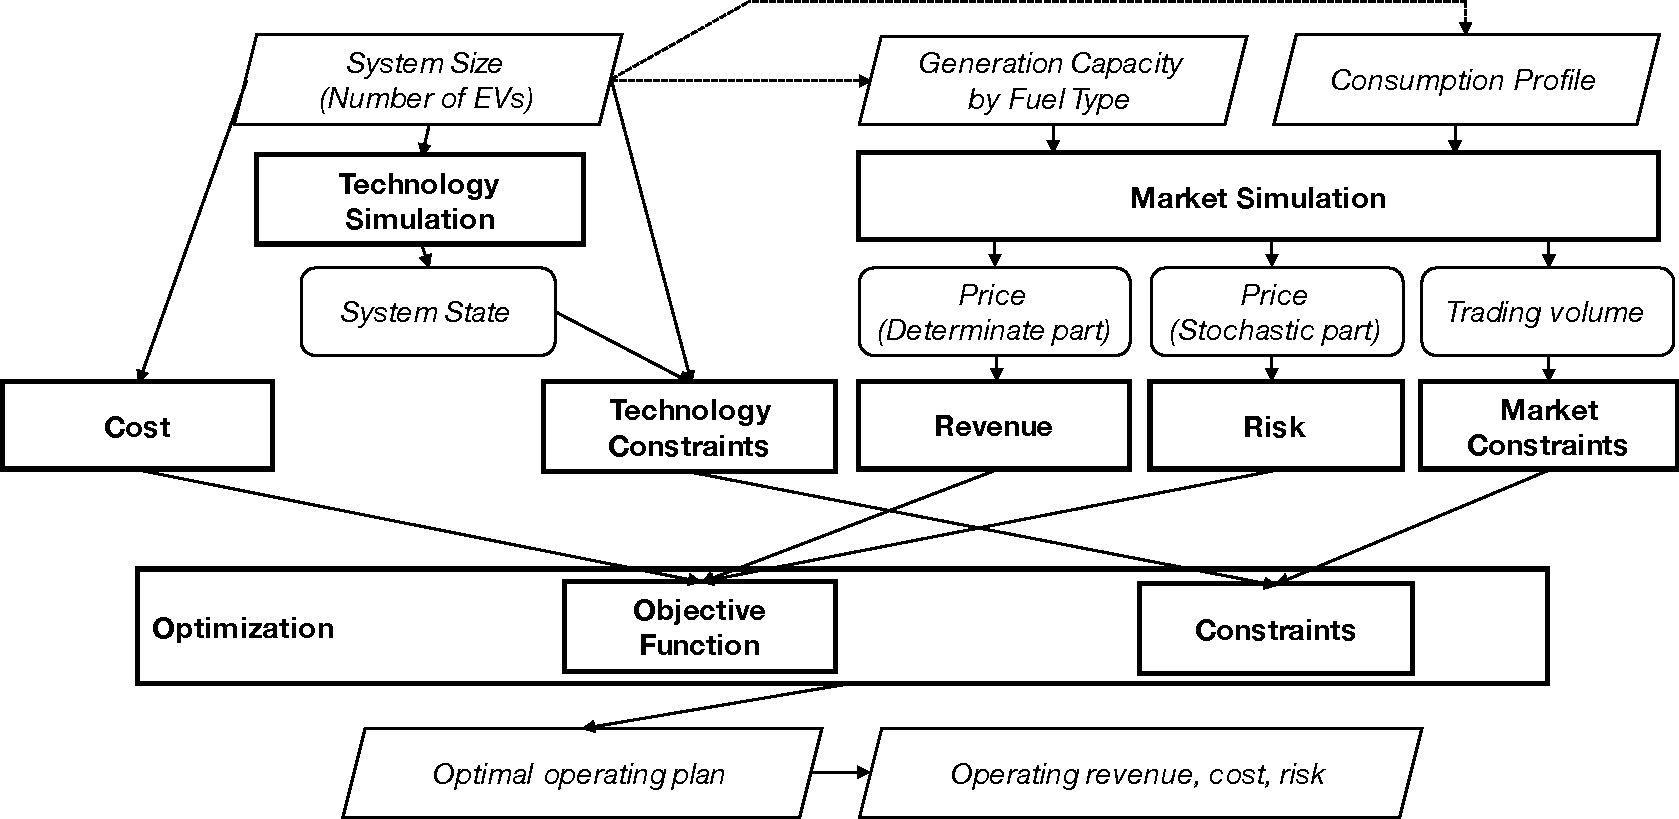
\includegraphics[scale=0.4]{Figures/ModelFlow.pdf}
	\caption{Flow chart of the techno-economic model}\
\end{figure}

Table \ref{tb:modules} offers an overview of all the modules and their inputs and outputs. The working flow of the model is illustrated by Figure \ref{fig:model-flow}.

With this model, we can evaluate the profitability and risk associated with a certain scale of flexibility management system in the power market and thus estimate the value of flexibility management market. Furthermore, we can assess the impact of driving factors including renewable penetration, cost reduction, and the possible diminishing return with increasing flexibility.

\section{Market-based modules}

\subsection{Revenue module}
\label{sec:revenue}
In this study, we only consider explicit revenues from power markets. At each time step ($t$), the revenue ($\text{REV}_t$) is calculate as the amount of energy ($e_t$, in MWh) offered in each energy market segment ($i$), and/or amount of reserve ($r_t$, in MW) offered in each reserve market segment ($j$), multiplied by their corresponding prices ($\pi_t$, in \$/MWh or \$/MW). In reserve market, there are additional revenues from energy provision while the committed capacities are activated. The amount of energy delivered in reserve market is determined as a proportion of the committed reserve using a term of ratio ($\delta_t$, in MWh/MW). The total revenue within a given period of time ($T$) and a set of selected energy markets ($I$) and a set of  selected reserve markets ($J$), can be then computed as:

\begin{equation}
\label{eq:module-revenue}
\text{REV}=  \sum_{t}^{t \in T} \text{REV}_t = \sum_{t}^{t \in T} \left( \sum_{i}^{i \in I}  \pi_t^{e,i} (e_t^{d,i} - e_t^{c,i})  + \sum_{j}^{j \in J} (\pi_t^{e,j} \delta_t^{j} + \pi_t^{r,j}) r_t^j \right)
\end{equation}

where, $d$ and $c$ in the superscripts denote "discharge" (to release energy from flexibility resources to grids) and "charge" (to intake energy from girds to flexibility resources) respectively.  $e_t^{d,i}$, $e_t^{c,i}$, $r_t^{j}$, are endogenous variables of the whole model and decision variables of the optimization, which represent the operation plan of the flexibility resource in power markets.

$I$ and $J$ are determined according to the business case being studied. For example, we can set $I = \{Day~ahead\}$ and $J=\emptyset$ in order to the value of making arbitrage in day-ahead energy market. 

If there are multiple elements in $I \cup J$, it means the flexibility resource can be reallocated to make offers to different market segments, i.e. performing multitasking. These cases need to be carefully managed to comply with actual market rules. Detailed treatments regarding multitasking are illustrated in section \ref{sec:special}.

The ratios $\delta_t$ are computed based on the real control signal when data is available, or otherwise using system average ratios between total activated energy ($\hat{e}_t^{r,j}$) and the total reserve ($\hat{e}_t^{r,j}$) at each time step.

%\begin{equation*}
%\delta_t^j = \frac{\hat{e}_t^{r,j}}{\hat{r}_t^j}
%\end{equation*}

Price signals, $\pi_t^{e,i}$, $\pi_t^{r,j}$ and $\pi_t^{e,j}$, are inputs for the revenue module and may be retrieved either directly from historical data or from the outputs of market simulation module described in Section \ref{sec:market-simulation}.

We re-formulate Equation \eqref{eq:module-revenue} in form as:

\begin{equation*}
\text{REV} = \textit{\textbf{f}}~X
\end{equation*}

where $X$ is the vector for all desicion variables. For certain sets of market segments $I$ and $J$, $X$ can be derived using Equations \eqref{eq:decision-variable-1} - \eqref{eq:decision-variable-end} with $i \in I$ and $j \in J$.
\begin{equation}
\label{eq:decision-variable-1}
X =
\begin{bmatrix}
E^d \\ E^c \\ R
\end{bmatrix}
\end{equation}

\begin{equation}
E^d =
\begin{bmatrix}
E^{d,I(1)} \\ \vdots \\ E^{d,i} \\ \vdots \\ E^{d,I(|I|)}
\end{bmatrix} \\
E^{d,i} = 
\begin{bmatrix}
e_1^{d,i}\\e_2^{d,i}\\\vdots\\e_T^{d,i}
\end{bmatrix}
\end{equation}

\begin{equation}
E^c =
\begin{bmatrix}
E^{c,I(1)} \\ \vdots \\ E^{c,i} \\ \vdots\\ E^{c,I(|I|)}
\end{bmatrix} \\
E^{c,i} = 
\begin{bmatrix}
e_1^{c,i}\\e_2^{c,i}\\\vdots\\e_T^{c,i}
\end{bmatrix}
\end{equation}

\begin{equation}
\label{eq:decision-variable-end}
R =
\begin{bmatrix}
R^{J(1)} \\ \vdots \\R^{j} \\ \vdots \\ R^{J(|J|)}
\end{bmatrix} ~~~\\
R^{j} = 
\begin{bmatrix}
r_1^{j}\\r_2^{j}\\\vdots\\r_T^{j}
\end{bmatrix}
\end{equation}

Function $\textbf{f}$ can be obtained analogously using Eqution \eqref{eq:decision-f-revenue-1} $\sim$ \eqref{eq:decision-f-revenue-end} with $i \in I$ and $j \in J$.
\begin{equation}
\label{eq:decision-f-revenue-1}
\textit{\textbf{f}} =
\begin{bmatrix}
\Pi^{e,I}~|~&-\Pi^{e,I}~|~&\Pi^{e,J} \Delta^J + \Pi^{r,J}
\end{bmatrix}
\end{equation}

\begin{equation}
\Pi^{e, I} =
\begin{bmatrix}
\Pi^{e,I(1)}~|~&\dots~|~&\Pi^{e,I(|I|)}
\end{bmatrix} ~~~\\
\Pi^{e,i} = 
\begin{bmatrix}
\pi_1^{e,i}~\pi_2^{e,i}~\dots~\pi_T^{e,i}
\end{bmatrix}
\end{equation}

\begin{equation}
\Pi^{e,J} =
\begin{bmatrix}
\Pi^{e,J(1)}~|~&\dots~|~&\Pi^{e,J(|J|)}
\end{bmatrix} ~~~\\
\Pi^{e,j} = 
\begin{bmatrix}
\pi_1^{e,j}~\pi_2^{e,j}~\dots~\pi_T^{e,j}
\end{bmatrix}
\end{equation}

\begin{equation}
\Pi^{r,J} =
\begin{bmatrix}
\Pi^{r,J(1)}~|~&\dots~|~&\Pi^{r,J(|J|)}
\end{bmatrix} ~~~\\
\Pi^{r,j} = 
\begin{bmatrix}
\pi_1^{r,j}~\pi_2^{r,j}~\dots~\pi_T^{r,j}
\end{bmatrix}
\end{equation}

\begin{equation}
\label{eq:decision-f-revenue-end}
\Delta^J = diag (
\delta_1^{J(1)}, \dots , \delta_T^{J(1)}, \dots, \delta_1^{J(|J|)}, \dots, \delta_T^{J(|J|)})
\end{equation}

%\subsection{Risk module}
In accordance with the revenue calculation, we consider the uncertain movement of price as the primary source of risk. Referring to similar works that performed risk management for flexibility sources, e.g. EV2G \cite{Alipour2017} and DER \cite{Han2017}, as well as for conventional energy trading companies \cite{Mohammadi-Ivatloo2013}, we developed a simple measure for risk control, by using the conditional value-at-risk (CVaR).

The CVaR (also named expected shortfall) as an extension of value-at-risk (VaR) can be defined as the difference between the expected profit and the average of potential profit values which are less than VaR \cite{Rockafellar2000}, shown as:

\begin{equation}
\label{eq:CVaR}
CVaR_\alpha (X) = \int_{\alpha}^{1} VaR_s(X) ds
\end{equation}

where $\alpha$ is the confidence level, and $X$ is the underlying (the price of energy/ reserve in our study). The VaR, as the negative of $\alpha$-quantile, can be computed as:

\begin{equation}
\label{VaR}
VaR_\alpha(X) = inf \{x \in \mathbb{R}~|~ P(X+x<0)\leq 1-\alpha\}
\end{equation}

Specially, in case the underlying variable subject to normal distribution, i.e. $X \sim \mathcal{N}(\mu,\,\sigma^{2})\,$, we can derive the CVaR as:

\begin{equation}
CVaR_\alpha(X) = \mu - \sigma \frac{\phi(\Phi^{-1}(\alpha))}{1-\alpha}
\end{equation}
%http://blog.smaga.ch/expected-shortfall-closed-form-for-normal-distribution/
where, $\Phi(\cdot)$ is cumulative distribution function and $\phi(\cdot)$ is the probability density function of normal distribution.

Alternatively, if the uncertainties are dealt with in a discrete manner, the CVaR can be calculated as\cite{Rockafellar2000}:

\begin{equation}
CVaR_\alpha (X) = \underset{\zeta}{max}\left( \zeta - \frac{1}{1-\alpha} \sum_{s} P(X,s) (\zeta - f(X,s))\right)
\end{equation}
where, $P(X,s)$ is the probability distribution function of $X$ in the scenario $s$ and $f(X,s)$ is the profit function in the scenario $s$. $\zeta$ is an auxiliary variable constrained by

\begin{equation*}
\zeta - f(X,s) \leq \zeta_s
\end{equation*}
\begin{equation*}
\zeta_s \geq 0
\end{equation*}

In our study, price terms $\tilde{\pi}$ are assumed to comprise a determinate part $\pi$ and an independent stochastic deviation $\epsilon$:
\begin{equation}
\label{eq:price-error}
\tilde{\pi_t}= \pi_t + \epsilon_t
\end{equation}

Since the stochastic terms $\epsilon$ are assumed to be uncorrelated to each other, the CVaR of our portfolio that is built by  $X^T = [E^d~|~E^c~|~R]$
in Equation \eqref{eq:decision-variable-1} can be aggregated as:

\begin{equation}
\begin{aligned}
CVaR =\sum_{t}^{t \in T} \{&\\
&\sum_{i}^{i \in I}  CVaR(\tilde{\pi_t}^{e,i}) (e_t^{d,i} - e_t^{c,i})  \\
&+ \sum_{j}^{j \in J} \left(CVaR(\tilde{\pi_t}^{e,j}) \delta_t^{j} + CVaR(\tilde{\pi_t}^{r,j})\right) r_t^j \\
&\}
\end{aligned}
\end{equation}

Analogous to the formation in preceding section, the risk module is also formulated in vector and matrix form.

\begin{equation*}
CVaR= \textit{\textbf{f}}
\begin{bmatrix}
E^d \\ E^c \\ R
\end{bmatrix}
\end{equation*}

where \textit{\textbf{f}} is calculated as:

\begin{equation}
\textit{\textbf{f}} =
\begin{bmatrix}
CVaR(\Pi^{e,I})\\-CVaR(\Pi^{e,I})\\CVaR(\Pi^{e,J}) \Delta^J + CVaR(\Pi^{r,J})
\end{bmatrix}^T
\end{equation}

\subsection{Market simulation module}
\label{sec:market-simulation}
As has been illustrated in the literature review (Chapter \ref{ch:LitRev}), valuation of flexibility with a dynamic market condition is still a challenging task. While investment decisions are extensively concerned with long-term trends, profitability of arbitrage sensitively depends on short-term price movement in high resolution. This is distinguishing from conventional electricity generators for whom a long-term forecast with coarse resolution is sufficient, and visual arbitrageurs who have almost no investments on infrastructures and may perform decision-makings with a short-term perspective. A holistic approach combining these researches were taken sometimes \cite{Rastler2010}\cite{Eyer2010} but may easily bring in unnecessary complexity and lead to an overwhelming demand of resources, which are not essential for our study.

Therefore, in this thesis, we customized a market model based on existing researches by re-focusing on factors that are most relevant to our research questions, and simplifying many other aspects of the power system and markets. Our market model is generally a statistic model built on observations of historical data, but a physical sub-model is incorporated as well to study the impacts of some relevant variables whose features are not well captured by empirical observations.

The approach for market simulation differentiates between energy markets and reserve markets. 

The energy markets are usually matured and with abundant degree of competition, so that we can employ an idealistic market model where the price formation is governed by the short run marginal costs (SRMCs) \cite{Grunewald2012} \cite{Grunewald2012a}. This allows us to leverage a merit-order model to simulate the price levels, which are widely adopted as is summarized in Chapter \ref{ch:LitRev}. 

The design of reserve markets, on the contrary, is not as straightforward as energy markets, which pose challenges for robust modeling. Besides, the market mechanisms vary spatially and temporally as is analyzed previously. Therefore, we adopt a pure statistic model for reserve market without involving any physical modeling.

\subsubsection{Day-ahead energy market}

The simulation for day-ahead energy market is preliminarily based on work done by \cite{Grunewald2012a} where the merit-order curve at supply shortage and surplus is modeled by an uplift effect. We further extend this work to capture the limits of flexibility provision in current energy markets so that we can simulate the market conditions when the flexibility become a challenge with growing renewables and/ or the flexibility becomes ubiquitous.

In \cite{Grunewald2012a}, the peak price during periods of high demand is explained as fewer participants remain with spare generating capacity, putting these actors in a stronger bidding position to mark up the price. In contrast, when demand is low and plants with high SRMCs would not operate so further reduction in generation would favor plants with low SRMCs and thus reverse the bidding position. In both cases, the less available capacity remains, the stronger bidding position for the remaining players, which happens at the two end of merit-order curve where the prices are driven up or down to significantly depart from the marginal cost. The symmetric effect is model with a uplift function:

\begin{equation}
U_t^g = 1 + \kappa~e^{-\alpha\left(\frac{C_t^g -P^g_t }{C^g}\right)}
\end{equation}

where $g$ denote the class of generation in merit order, e.g. peak, flexible, inflexible, etc. ($\kappa$) and ($\alpha$) are the parameters which can be obtained empirically \cite{Cox2009}. In case of peak period, $C^g_t$ represents total avaiable generation capacity of class $g$ and $P^g_t$ is the output of genertion of class g. During period of generation surplus, $C^g_t$ is the remaining generation capacity while $P^g_t$ is the curtailment required.

The middle of merit order curve can be modeled with a linear relationship.

Since the SRMCs of renewable generations are almost zero or even negative when they are remunerated by renewable support schemes, their position in power market is distinguishing from other generation players. Therefore, we employed the residual load, i.e. the load net of renewable generation, which has been introduced previously. We denote the residual load as $L^{res.}$ here.

According to the discussion above, the uplifts will occur when $L^{res.}$ exceeds the capacity of mid-merit generations and when $L^{res.}$ is smaller than operating capacity of inflexible generations.

Therefore, the merit order model for price formation can be formulated as:

\begin{equation}
\label{eq:merit-order-model}
\pi_t = \begin{cases}
\dot{\pi}_t \left[1 + \kappa~e^{-\alpha\left(\frac{C_t^g -P^g_t }{C^g}\right)} \right] & L^{res.}_t \leq C^{inflex.}_t\\ 
\dot{\pi}_t ~\kappa~\frac{P^g_t}{C_t^g} & C^{inflex.}_t < L^{res.}_t < C^{inflex.}_t+ C^{mid.}_t\\
\dot{\pi}_t  \left[1 + \kappa~e^{-\alpha\left(\frac{C_t^g -P^g_t }{C^g}\right)} \right] & L^{res.}_t \geq C^{inflex.}_t + C^{mid.}_t\\
\end{cases}
\end{equation}

In order to derive the value of generation capacity of each class, an investigation into the flexibility of power plants is necessary.

\begin{figure}[h!]
	\label{fig:power-plant-flexibility}
	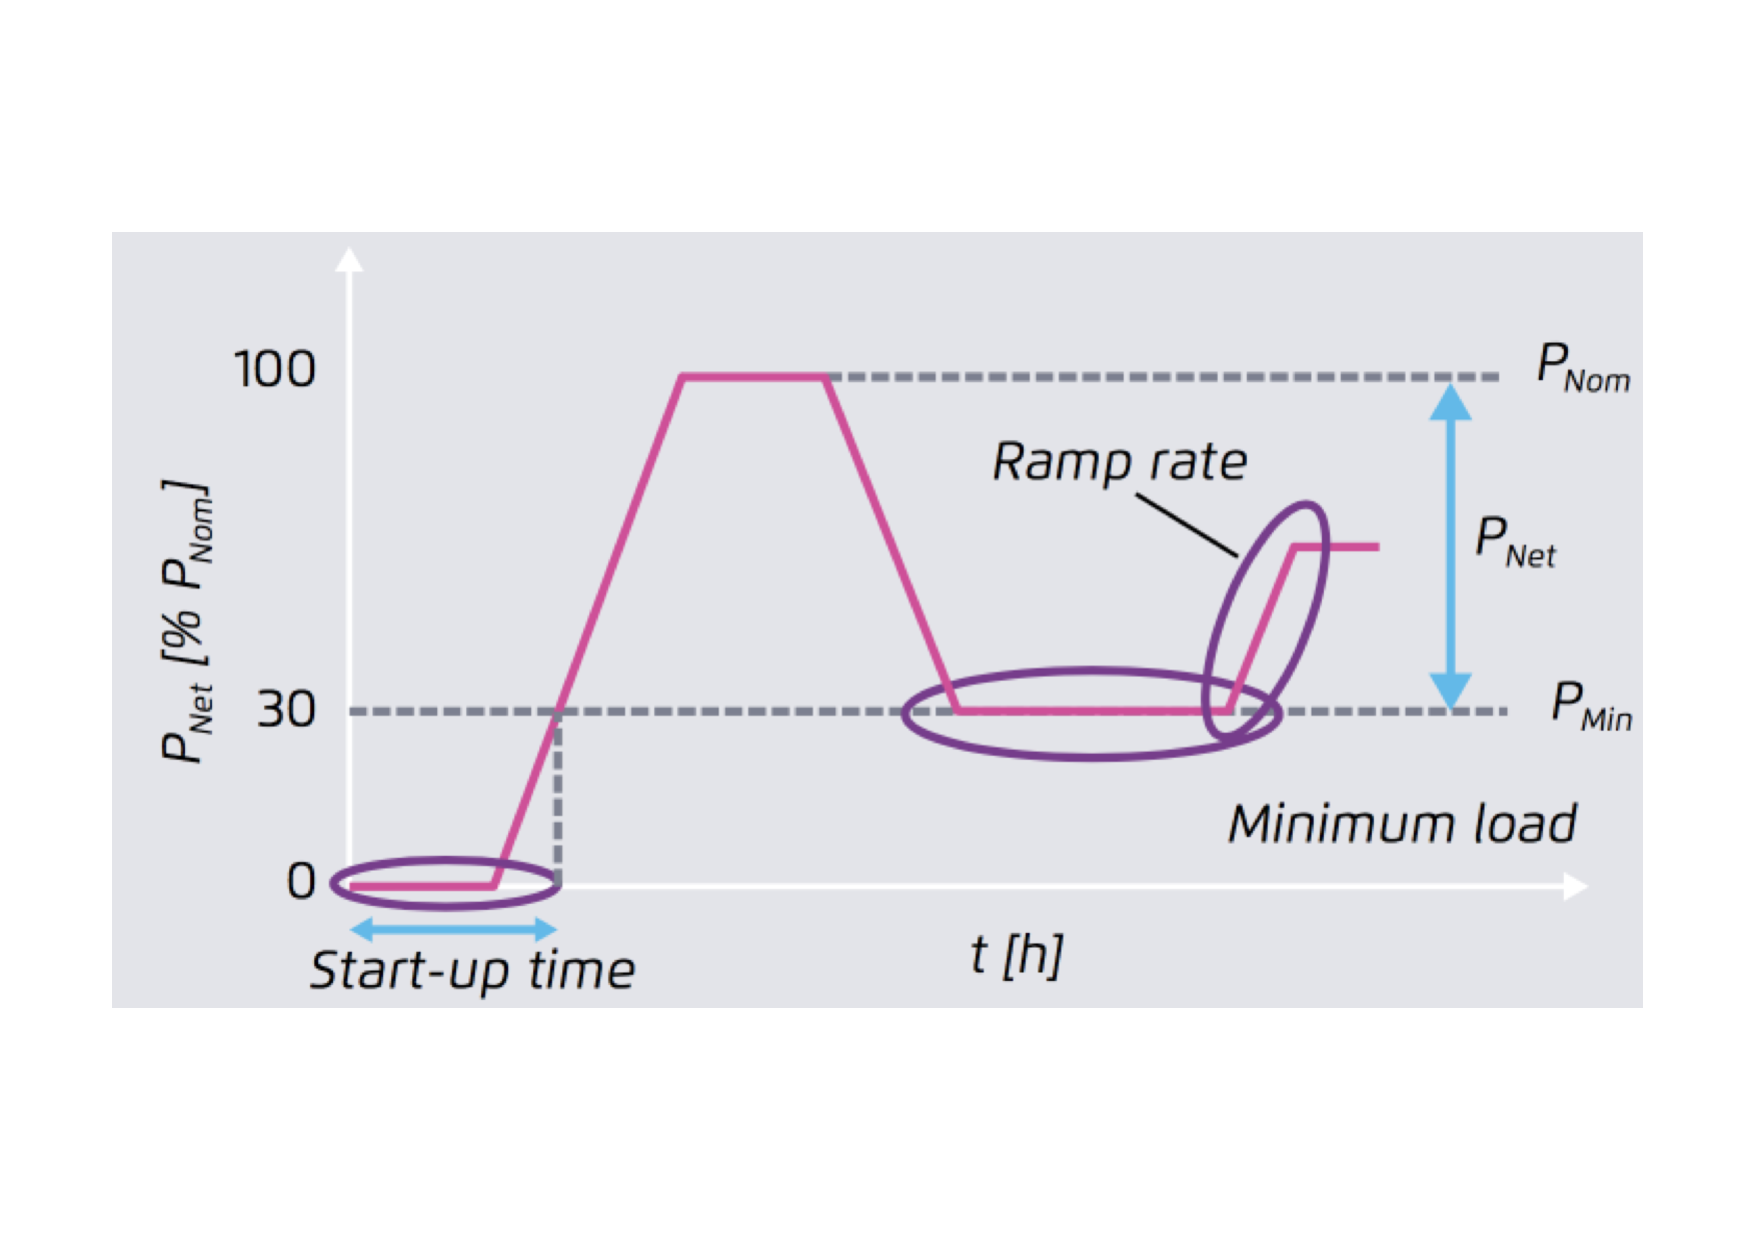
\includegraphics[scale=0.4]{Figures/PowerPlantFlexibility.pdf}
	\caption{Qualitative representation of key flexibility parameters of a power plant\cite{AgoraEnergiewende2017}}\
\end{figure}

The flexibility of a power plant can be characterized by three key features\cite{AgoraEnergiewende2017} (Figure \ref{fig:power-plant-flexibility}): 
\begin{itemize}
	\item Overall bandwidth of operation: the range of output between minimum and maximum load;
	\item Ramp rate: the speed of adjusting output;
	\item Start-up time: the time required to attain stable operation from standstill
\end{itemize}

%https://www.researchgate.net/profile/Alejandro_Hoese
If a power plant can adjust its load from zero to nominate capacity within a time block in the day-ahead market (typically 1 hour), it can be deemed with infinite flexibility in the day-ahead market. This applies to most type generations including solar, wind, hydro and electrochemical systems, etc., except for generations using steam turbines \cite{AgoraEnergiewende2017}, including nuclear, coal-, oil and gas-steam, etc. The gas turbines can be ramped up to full capacity within typically 30 minutes\cite{Siemens}\cite{GE} so can be considered as flexible generation.

For a steam-turbine power plant, the minimum operational load is about 25-60\% of its nominal capacity while the time required to start from standstill is longer than 2 hours \cite{AgoraEnergiewende2017}. Therefore, they are treated as limited flexible sources.

For limited flexible generations, an empirical analysis is performed to determine its bounded flexibility. The procedure for a certain generation source is decribed as following and shown as Figure \ref{fig:bounded-flexibility}:

\begin{figure}[h!]
	\label{fig:bounded-flexibility}
	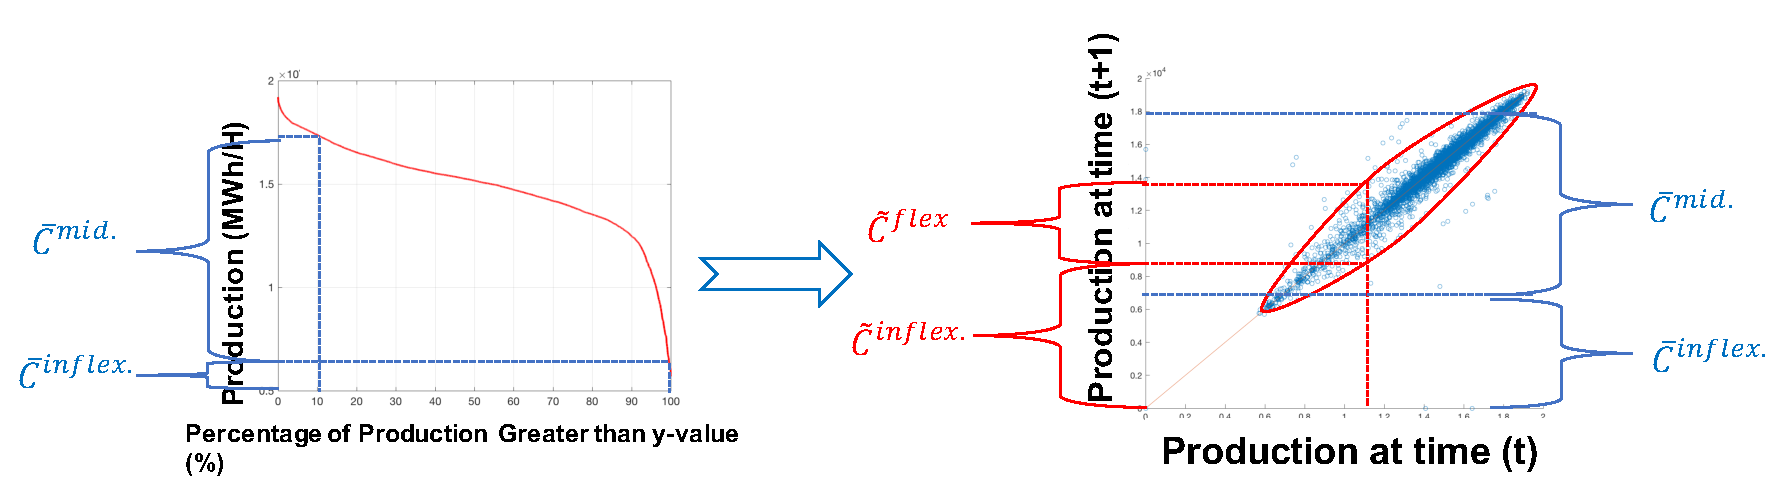
\includegraphics[scale=0.4]{Figures/BoundedFlexibility.pdf}
	\caption{Schematic illustration of determining bounded flexibility for limited flexible generations}\
\end{figure}


\begin{enumerate}
	\item Make the duration curve of the generation data, and obtain $\overline{c}^{mid.}$ which is the range that the generation source is operating for over 10-99\% of the overall period and $\overline{c}^{inflex.}$ which is the range that the generation is operating of more than 99\% of the time.
	\item Determine the envelop lines which limit the production at time $t+1$ based on production at time $t$. With a certain production $p_{t}$, $p_{t+1}$ is bounded within $\tilde{c}^{flex}$, and there is a range of production $\tilde{c}^{inflex}$ that is not economically viable to be curtailed.
	\item Finally, we find the relationship that map the production at time $t$ to flexible capacity at time $t+1$ as: 
	\begin{equation}
	\begin{aligned}
	c^{inflex.}_{t+1} &= \mathcal{C}^{inflex}(p_t)\\ &=max\{\tilde{c}^{inflex.}_t,~\overline{c}^{inflex.}\}
	\end{aligned}
	\end{equation}
	\begin{equation}
	\begin{aligned}
	c^{flex.}_{t+1} &= \mathcal{C}^{flex.}(P_t) \\ & =min\{\tilde{c}^{flex.}_t+\tilde{c}^{inflex.}_t,~\overline{c}^{mid.}+\overline{c}^{flex}_t \} - \tilde{c}^{inflex.}_t
	\end{aligned}
	\end{equation}
	\begin{equation}
	\begin{aligned}
	c^{peak}_{t+1} &= \mathcal{C}^{peak}(P_t) \\ & =max\{\tilde{c}^{flex.}_t+\tilde{c}^{inflex.}_t -(\overline{c}^{mid.}+\overline{c}^{flex}_t),0 \}
	\end{aligned}
	\end{equation}
\end{enumerate}

When the load exceeds the flexible range of these sources, they are no long able to participate in the bidding so these portion of capacity shall be deducted from the overall capacity for the calculation using Equation \eqref{eq:merit-order-model}.

Finally, a regression is performed to determine the parameters in Equation \eqref{eq:merit-order-model} using empirical observations. The errors between a regressed value $\pi_t$ and an actual value $\tilde{\pi}_t$ would be analyzed as the uncertainty of price movement and used for risk controlling as is discussed in risk module. 

With a established merit-order model for day-ahead energy market, we can re-simulate the price with changed market condition, e.g. altered generation capacity mix.

\subsubsection{Real-time energy market and reserve market}

In electricity markets, large portion of energy is usually traded in day-ahead market \cite{Kardakos2013}. There are significate dependences of the real-time (intraday, balancing) energy price on day-ahead price \cite{Woo2016}. Therefore, for real-time energy prices, we adopt a simplex empirical analysis based on comparing the results from day-ahead price simulation and actual market data:

\begin{equation}
\pi^{RT}_t = \kappa (\pi^{DA}_t + \alpha) + \epsilon_t
\end{equation}
where, $\kappa$ and $\alpha$ are terms to adjust the determinate bias between day-ahead and real-time price, while $\epsilon_t$ represents the stochastic movement of real-time price. 

For reserve market, only an empirical model is used as is discussed previously.

\subsection{Market constraints}

The market constraints are a list of limits to make sure that the operation of flexibility resource (determined by $X$ in Equation \eqref{eq:decision-variable-1}) would not violate the actual market rules and market conditions.

Generally, these constraints can be formulated as

\begin{equation}
\begin{bmatrix}
\Gamma^d~~|& \Gamma^c~~|&\Gamma^r
\end{bmatrix}
X \leq \textit{\textbf{b}}
\end{equation}

Most of the market constraints are derived from the market rules so will be introduced in case studies where specific markets are being studies. 

%Capacity constraints:
%\begin{equation}
%r_t^j \leq \hat{r}_t^j ~~~ j \in J
%\end{equation}

%Since in this study high penetration of flexibility resources will be investigated, 

%Day-ahead
%\begin{equation}
%\hat{e}_t^i - \hat{e}_t^{peak} \leq e_t^{d,i} - e_t^{c,i} \leq \hat{e}_t^i - \hat{e}_t^{base} ~~~ i \in \{Day~Ahead\}
%\end{equation}

%Real-time
%PJM revised order +/- 10% of the DA offer
%Germany volume limited





\section{Technology-based modules}

\subsection{Cost module}
\label{sec:cost}
In this thesis, we categorize all costs into two groups: operation-independent and operation-dependent costs.

\subsubsection{Operation-independent costs}
The first group mainly including the initial capital outlay for purchasing the devices and systems, plus the fixed operating and maintenance (O\&M) costs which include miscellaneous items such as the insurance, employee salaries, etc. 

The initial capital cost for a storage system can be divided into two components: an energy-based component, approximately linear to the energy capacity of the system (denoted $\overline{s}$, in MWh), and a power-based component, approximately linear to the power rate of the system (denoted $\overline{r}$, in MW) \cite{Megel2017}. Additionally, we add a component representing the size-invariant costs such as the cost for software. Thereby, the initial capital cost can be computed as:

\begin{equation}
\label{eq:initial-cost}
C^{ini} = C^s \overline{s} + C^r \overline{r} + C^0
\end{equation}

where, the coefficients can be obtained empirically either by screening actual market data or from literature. In addition, since the system cost for battery storage is falling rapidly, a learning rate of \textit{ca.} 14\% per annum can be taken to build future scenarios\cite{Nykvist2015}.

The initial capital cost is then annualized by using the concept of equivalent annual cost (EAC):

\begin{equation}
C^{EAC} = \frac{C^{ini}}{\frac{1 - \frac{1}{(1+r)^a}}{r}}
\end{equation}

where $r$ is the discount rate and $a$ is the lifespan of the system in number of years.

The discount rate can be established from the Weighted Average Cost of Capital (WACC) which depends on the financial conditions of different players. A typical WACC in the United States is \textit{ca.} 4-6\% for a municipal utility, 7-8\% for a regulated utility and over 10\% for independent power producer\cite{Rastler2010}. In this study, a discount rate of 10\% is taken unless otherwise stated.

For fixed O\&M costs, $C^{fO\&M}$ which is difficult to calculate precisely, an assumption of 2\% of the initial capital cost is taken, referring to \cite{Rastler2010}. The fixed O\&M costs are added directly to the annualized capital cost to get the total fix costs (in \$/year):

\begin{equation}
C^{fix} = C^{EAC} +  C^{fO\&M}
\end{equation}

The annualized fix cost will finally be compared with the operating revenue calculated from other module to assess the profitability.

\subsubsection{Operation-dependent costs}

Operation-dependent costs primarily refer to the degradation costs, which is specially an issue for battery-based energy storage systems\cite{Barre2013}.

However, as has been reviewed and analyzed in \cite{Megel2017}, there exists no single degradation model that is widely accepted among the literature and applicable for all cases, due to the complexity of this problem. The reasons can be summarized as following:
\begin{itemize}
	\item Modelling battery degradation itself is a complex engineering problem as it is affected by a list of physical parameters, including the degree-of-discharge (DoD), state-of-charge (SoC), charging/discharging rate, temperature, etc.\cite{Barre2013}
	\item The choice of degradation model affects the convex relaxation when degradation effects are included in an optimization problem, the model selection is driven by the requirements of mathematical realization. \cite{Megel2017}
\end{itemize}

Degradation costs can be neglected while operating life time is longer than designed life time, which is generally valid for non-battery energy systems \cite{Bradbury2014}\cite{Zafirakis2016}\cite{Connolly2011}. Some research works studying battery system also made the same assumption  \cite{Byrne2012}\cite{McConnell2015}\cite{Sioshansi2009}. The breakeven point of operational frequency where the degradation of battery storage system can be ignored was concluded to be less than 0.5-1.5 full-cycle equivalent energy throughput per day\cite{Megel2017}. Nonetheless, it was also pointed out by \cite{Megel2017} that while assuming degradation cost being zero, the operational planner would tend to operate the system more frequently, which would possibly in turn to violate the assumption of zero-degradation.

Such a combined investment and operation problem is hard to be incorporated in an optimization, so in our study we first use a simple degradation cost model where the cost is linear to the \textit{energy throughput} $|e^t|$ as a damping term in the optimization and examine it \textit{ex-post}, i.e. if the actual operating life is not reached the degradation cost will be exempted from the final profit calculation. A linear relationship between the degradation and $|e^t|$ is a common technique used in researches for estimating battery degradation\cite{Byrne2012}\cite{Berrada2016}.

Denoting the damping factor for degradation as $\zeta$, we can formulate the degradation damping as:

% THIS IS WRONG
\begin{equation}
\label{eq:degradation-damping}
C^{degradation}_t = \zeta (\sum_{i}^{i \in I}(e_t^{d,i}+e_t^{c,i})+\sum_{j}^{j \in J}(\delta_t^{j,+}+\delta_t^{j,-})r_t^j)
\end{equation}

where, the energy to reserve ratios are separated to positive and negative components:
\begin{equation}
\label{eq:ratio-pos}
\delta_t^{j,+} = \begin{cases}
\delta_t^j & \delta_t^j  \geq 0\\
0 & \delta_t^j  < 0
\end{cases}
\end{equation}
\begin{equation}
\label{eq:ratio-neg}
\delta_t^{j,-} = \begin{cases}
0 & \delta_t^j  \geq 0\\
-\delta_t^j & \delta_t^j  < 0
\end{cases}
\end{equation}

It can be noticed that when a virtual arbitrage is conducted where some $e_t^{d,i}$ and $e_t^{c,i}$ are offset, it will activate the degradation damping with Equation \eqref{eq:degradation-damping} while there are no real physical processes causing degradation. This will be corrected in final profit calculation but in decision making process using optimizations we keep it as it is intended to restrict the virtual arbitrage.

Similar to Equation \eqref{eq:decision-f-revenue-end}, we reconstruct the diagonal matrices with the decomposed ratios from Equation \eqref{eq:ratio-pos} and \eqref{eq:ratio-neg}.
\begin{equation}
\Delta^+ = diag (
\delta_1^{J(1),+}, \dots , \delta_T^{J(1),+}, \dots, \delta_1^{J(|J|),+}, \dots, \delta_T^{J(|J|),+})
\end{equation}
\begin{equation}
\Delta^- = diag (
\delta_1^{J(1),-}, \dots , \delta_T^{J(1),-}, \dots, \delta_1^{J(|J|),-}, \dots, \delta_T^{J(|J|),-})
\end{equation}

The matrix of coefficient for degradation is the derived complying with the form of market modules:

\begin{equation*}
Cost^{degradation} = \begin{bmatrix}
Z^{I}~|~&Z^{I}~|~& \zeta (\Delta^{+} +\Delta^{-})
\end{bmatrix} \begin{bmatrix}
E^d \\ E^c \\ R
\end{bmatrix}
\end{equation*}

where,
\begin{equation*}
Z^I = \begin{bmatrix}
Z^{I(1)}~~|&\dots~~|&Z^i~~|&\dots~~|&Z^{I(|I|)}
\end{bmatrix}~~~
Z^i = \zeta \cdot I_{T\times T} ~~~ \forall i \in I
\end{equation*}

$I_{T \times T}$ is a ($T \times T$) identity matrix. 

\subsection{Technology simulation module}
\label{sec:tech-simulation-module}
The technology simulation is applied to determine the state of the system, which would be used primarily for calibration of technology constraints but also for \textit{ex-post} analysis.

\subsubsection{Energy Storage}
Regardless of the type of technology, an energy storage system consists of three functional units, i.e. power input, power output, and storage. Each function unit is associated with an efficiency, i.e. conversion efficiencies of charging, discharging and storage efficiency, denoted as $\eta_c$, $\eta_d$ and $\eta_s$ respectively.

Since the ramp up time for a typical storage system is neglectable comparing to the time resolution in our study, the state of power input and output are deemed as strictly following the operational plan without transient process.

For the state of storage, we define a term, $s$ (in MWh), which is the energy stored in the device, i.e. the State-of-Charge (SoC) multiplied by its maximum energy capacity. The state is determined using Equation \ref{eq:tech-ESS}.

\begin{equation}
\label{eq:tech-ESS}
s_t = \eta_s s_{t-1} + \eta_c (\sum_{i}^{i \in I} e_t^{c,i} + \sum_{j}^{j \in J}\delta_t^{j,-}r_t^j)- \frac{1}{\eta_d} (\sum_{i}^{i \in I} e_t^{d,i} + \sum_{j}^{j \in J}\delta_t^{j,+}r_t^j)
\end{equation} 

In order to formulate Equation \eqref{eq:tech-ESS} in matrix form, we first introduce a matrix denoted $H$:
\[
H
=
\begin{bmatrix}
\eta_s^0 & 0 & 0 &  \dots & 0 \\
\eta_s^1 & \eta_s^0 & 0 &  \dots & 0 \\
\eta_s^2 & \eta_s^1 & \eta_s^0 &  \dots & 0 \\
\vdots & \vdots & \vdots &  \ddots & \vdots \\
\eta_s^{T-1} & \eta_s^{T-2} & \eta_s^{T-3} & \dots & \eta_s^0 \\
\end{bmatrix}
\]
\newline
Then $M$ is used to construct $H^I$ and $H^J$ with a given pair of sets of market segments $I$ and $J$.
\begin{equation*}
H^I = \begin{bmatrix}
H^{I(1)}~~|&\dots~~|&H^i~~|&\dots~~|&H^{I(|I|)}
\end{bmatrix}~~~
H^i = H ~~~ \forall i \in I
\end{equation*}
\begin{equation*}
H^J = \begin{bmatrix}
H^{J(1)}~~|&\dots~~|&H^j~~|&\dots~~|&H^{J(|J|)}
\end{bmatrix}~~~
H^j = H ~~~ \forall j \in J
\end{equation*}
Finally, we can derive the matrix form of Equation \eqref{eq:tech-ESS}.
\begin{equation}
\label{eq:tech-ESS-M}
S = \eta_s H S_0 + \begin{bmatrix}
-\frac{1}{\eta_d} H^I~~|& \eta_c H^I~~|& H^J (-\frac{1}{\eta_d} \Delta^{+} + \eta_c \Delta^{-})
\end{bmatrix} X
\end{equation}
where, $S$ and $S_0$ are vectors for the temporal and initial state, respectively.
\begin{equation*}
S = \begin{bmatrix}
s_1~~s_2~~\dots~~s_T
\end{bmatrix}^T
\end{equation*}
\begin{equation*}
S_0 = \begin{bmatrix}
s_0~~s_0~~\dots~~s_0
\end{bmatrix}^T
\end{equation*}

In order to make it more compact, we reformulate Equation \eqref{eq:tech-ESS-M} as:

\begin{equation}
\label{eq:state-ESS-M-1}
S = \textit{\textbf{h}}_0 + \textit{\textbf{h}}~X
\end{equation}
where
\begin{equation}
\label{eq:state-ESS-M-2}
\textit{\textbf{h}}_0 =  \eta_s H S_0
\end{equation}
\begin{equation}
\label{eq:state-ESS-M-3}
\textit{\textbf{h}} = \begin{bmatrix}
-\frac{1}{\eta_d} H^I~~|& \eta_c H^I~~|& H^J (-\frac{1}{\eta_d} \Delta^{+} + \eta_c \Delta^{-})
\end{bmatrix}
\end{equation}
\subsubsection{Electric Vehicle}

Electric vehicle to grid systems are fundamentally battery energy storage systems in term of their physical dynamics. Therefore, they can be modeled generally using the same approach as in preceding paragraphs. However, there are several attributes that uniquely characterize electric vehicle to grid systems compared to normal battery storage:

\begin{itemize}
	\item The availability of an EV2G system, in terms of delivering both energy (in MWh) and capacity reserve (in MW), is dynamic rather than static, since the number of EVs connected in the power grid is changing all the time with the behaviors of plug-in/ plug-out.
	\item The energy stored in the system will be consumed not only for delivering our targeted services (arbitrage or balancing), but also for driving of EVs themselves. This part of costs will be implicitly captured by the revenue module using Equation \eqref{eq:module-revenue}, which will distort the real value of services provided for the grid. 
\end{itemize}

Therefore, two main modifications are made to adapt the model of ESSs for better representing the EV2G systems: 

\begin{enumerate}
	\item The EV2G system is modeled as a dynamic ESS by taking into consideration the connection/ disconnection of EVs to/ from the grids.
	\item The costs of energy consumed for driving are accounted and analyzed separately
\end{enumerate}

It shall be noticed with the dynamic storage model, only the overall state on the whole system level, i.e. the aggregation of all EVs in the system, is monitored and complied with the technological constraints. Performing simulation and optimization for each EV with a distributed approach is beyond the scope of this study. 

In order to transform the model for ESS to be dynamic in size and availability, we introduce additional terms to represent the number of EVs entering ($n_t^+$), leaving ($n_t^-$) and remain in ($n_t$) the system at each time step.
\begin{equation}
\label{eq:EV-number}
n_t = n_{t-1} + n_t^+ - n_t^-
\end{equation}

The energy stored in each EV while being plugged-in or plugged-out are denoted as $s_t^+$ and $s_t^-$, respectively. $n_t^+$, $n_t^-$, $s_t^+$ and $s_t^-$ can be determined statistically from real vehicle driving profiles. 

Thereby the state equation for an EV2G system is written as:
\begin{equation}
\label{eq:tech-EV}
\begin{aligned}
s_t = & \eta_s s_{t-1} + \eta_c (\sum_{i}^{i \in I} e_t^{c,i} + \sum_{j}^{j \in J}\delta_t^{j,-}r_t^j)- \frac{1}{\eta_d} (\sum_{i}^{i \in I} e_t^{d,i} + \sum_{j}^{j \in J}\delta_t^{j,+}r_t^j) \\
&+ s_t^+ n_t^+ - s_t^- n_t^-
\end{aligned}
\end{equation} 
\newline
The matrix form of Equation \eqref{eq:EV-number} is as following:
\begin{equation}
\label{eq:EV-number-M}
N = I_{T \times T} N_0 + L_{T \times T} N^+ -L_{T \times T} N^- 
\end{equation}
where, $L_{T \times T}$ is a ($T \times T$) identity lower triangular matrix. The rest matrices are defined as following
\begin{equation*}
N = \begin{bmatrix}
n_1~~n_2~~\dots~~n_T
\end{bmatrix}^T
\end{equation*}
\begin{equation*}
N_0 = \begin{bmatrix}
n_0~~n_0~~\dots~~n_0
\end{bmatrix}^T
\end{equation*}
\begin{equation*}
N^+ = \begin{bmatrix}
n_1^+~~n_2^+~~\dots~~n_T^+
\end{bmatrix}^T
\end{equation*}
\begin{equation*}
N^- = \begin{bmatrix}
n_1^-~~n_2^-~~\dots~~n_T^-
\end{bmatrix}^T
\end{equation*}
\begin{equation*}
S^+ = diag(s_1^+, s_2^+, \dots, s_T^+
)
\end{equation*}
\begin{equation*}
S^- = diag(s_1^-, s_2^-, \dots, s_T^-)
\end{equation*}
\newline
Analogously, translating Equation \eqref{eq:tech-EV} to matrix form leads to:

\begin{equation}
\begin{aligned}
S = &~ \eta_s H S_0 + H S^+ N^+ - H S^- N^- \\
&~+ \begin{bmatrix}
-\frac{1}{\eta_d} H^I~~|& \eta_c H^I~~|& H^J (-\frac{1}{\eta_d} \Delta^{+} + \eta_c \Delta^{-})
\end{bmatrix} X
\end{aligned}
\end{equation}
which can be reformulated as:
\begin{equation}
\label{eq:state-EV-M-1}
S = \textit{\textbf{h}}_0 + \textit{\textbf{h}}~X
\end{equation}
where
\begin{equation}
\label{eq:state-EV-M-2}
\textit{\textbf{h}}_0 =  \eta_s H S_0 + s^+ H N^+ - s^- H N^-
\end{equation}
\begin{equation}
\label{eq:state-EV-M-3}
\textit{\textbf{h}} = \begin{bmatrix}
-\frac{1}{\eta_d} H^I~~|& \eta_c H^I~~|& H^J (-\frac{1}{\eta_d} \Delta^{+} + \eta_c \Delta^{-})
\end{bmatrix}
\end{equation}

\subsection{Technology constraints}
\label{sec:tech-constraints}
The technology constraints are set to ensure the operation plan is fulfilled physically by the system.

\subsubsection{Energy storage}
Firstly, the charging/ discharging rate shall be bounded at its maximum rate ($\overline{r}$, assuming symmetric for charge and discharging).

\begin{equation}
0 \leq \frac{1}{\Delta t}\sum_{i}^{i \in I} e^{d,i}_t + \sum_{j}^{j \in J} r_t^j \leq \overline{r}~~~ \forall t \in T
\end{equation}

\begin{equation}
0 \leq \frac{1}{\Delta t}\sum_{i}^{i \in I} e^{c,i}_t + \sum_{j}^{j \in J} r_t^j \leq \overline{r}~~~ \forall t \in T
\end{equation}

It can be noticed that opposite movement of charging/ discharging in different markets are not offset in the constraints. This implies virtual arbitrageurs are not allowed to make deals that cannot be afforded physically although the physical systems are not actually activated.

Meanwhile, the energy stored is restricted as well.

\begin{equation}
0 \leq s_t \leq \overline{s}~~~ \forall t \in T
\end{equation}

Replacing $s_t$ using Equation \eqref{eq:tech-ESS}, the contraint is formulated as:
\begin{equation}
0 \leq \eta_s s_{t-1} + \eta_c (\sum_{i}^{i \in I} e_t^{c,i} + \sum_{j}^{j \in J}\delta_t^{j,-}r_t^j)- \frac{1}{\eta_d} (\sum_{i}^{i \in I} e_t^{d,i} + \sum_{j}^{j \in J}\delta_t^{j,+}r_t^j) \leq \overline{s}
\end{equation}

Applying the matrix format of the equations, we can get the constraints re-formulated the constraints of rates as:

\begin{equation}
- \frac{1}{\Delta t} \begin{bmatrix}
\overbrace{ I_{T\times T}|\dots|I_{T\times T}}^\text{|I|}|\overbrace{O_{T\times T}|\dots|O_{T\times T}}^\text{|I|}|\overbrace{ I_{T\times T}|\dots|I_{T\times T}}^\text{|J|}| 
\end{bmatrix} X \leq 0
\end{equation}

\begin{equation}
- \frac{1}{\Delta t} \begin{bmatrix}
\overbrace{ O_{T\times T}|\dots|O_{T\times T}}^\text{|I|}|\overbrace{I_{T\times T}|\dots|I_{T\times T}}^\text{|I|}|\overbrace{ I_{T\times T}|\dots|I_{T\times T}}^\text{|J|}| 
\end{bmatrix} X \leq 0
\end{equation}

\begin{equation}
\label{constraint:ESS-capacity}
\frac{1}{\Delta t} \begin{bmatrix}
\overbrace{ I_{T\times T}|\dots|I_{T\times T}}^\text{|I|}|\overbrace{O_{T\times T}|\dots|O_{T\times T}}^\text{|I|}|\overbrace{ I_{T\times T}|\dots|I_{T\times T}}^\text{|J|}| 
\end{bmatrix}X \leq \overline{R}
\end{equation}
\begin{equation}
\label{constraint:ESS-capacity-2}
\frac{1}{\Delta t} \begin{bmatrix}
\overbrace{ O_{T\times T}|\dots|O_{T\times T}}^\text{|I|}|\overbrace{I_{T\times T}|\dots|I_{T\times T}}^\text{|I|}|\overbrace{ I_{T\times T}|\dots|I_{T\times T}}^\text{|J|}| 
\end{bmatrix}X \leq \overline{R}
\end{equation}

where $O_{T \times T}$ is a $T \times T$ zero matrix and
\begin{equation*}
\overline{R} = \begin{bmatrix}
\overbrace{\overline{r}, \dots, \overline{r}}^\text{T}
\end{bmatrix}^T
\end{equation*}


The constraints of storage are formulated as:
\begin{equation}
\label{constraint:ESS-energy-1}
-\textit{\textbf{h}}~X \leq \textit{\textbf{h}}_0
\end{equation}
\begin{equation}
\label{constraint:ESS-energy-2}
\textit{\textbf{h}}~X \leq \overline{S} -  \textit{\textbf{h}}_0
\end{equation}
where, $\textit{\textbf{h}}$ and $\textit{\textbf{h}}_0$ are determined by Equation \eqref{eq:state-ESS-M-1} to \eqref{eq:state-ESS-M-3}, and
\begin{equation*}
\overline{S} = \begin{bmatrix}
\overbrace{\overline{s}, \dots, \overline{s}}^\text{T}
\end{bmatrix}^T
\end{equation*}

\subsubsection{Electric vehicle to grid}

The constraints for ESS are generally portable for the EV2G systems, by simplying re-using Equation \eqref{eq:state-EV-M-1} to \eqref{eq:state-EV-M-3} to derive $\textit{\textbf{h}}$ and $\textit{\textbf{h}}_0$, and replacing the upper bound limit in Equation \ref{constraint:ESS-capacity} with

\begin{equation}
\overline{R} = \overline{r}N
\end{equation}
where, $N$ is determined by Equation \eqref{eq:EV-number-M}. 




\section{Optimization Engine}
The performance of a flexibility resource depends primarily on the operation plan, which is represented as $X$ (Equation \ref{eq:decision-variable-1}). In order to value the market of technology vendors supplying flexibility to actors in power markets, we need to find reasonable operation patterns that simulate the behaviors of those players. For this sake, we employ an optimization engine. The value of market calculated with the results from optimization stands for the upper bound of market value.

The objective function of the optimization problem is formulated as:
\begin{equation}
\underset{X}{max} \left[ (1-\beta)\left(Revenue (X) - C^{degradation}(X)\right) - \beta CVaR(X) \right]
\end{equation}
where, X is the vector of decision variables (Equation \eqref{eq:decision-variable-1}), and $Revenue$, $C^{degradation}$ and $CVaR(X)$ are calculated using the equations in corresponding modules. $\beta$ is a weighting parameter with $\beta \in [0,1]$, which is used to study the trade-off between profit and risk.

The constraints have been introduced in the modules of market and technology constraints.

The optimization is implemented in MATLAB\textcopyright~and solved using Guobi optimizer. 

\section{Addtional measures for special cases}
\label{sec:special}

\subsection{Backcast technique to reduce the predictability of price}
As has been discussed in the literature review, many of the researches on arbitrage of flexibility in power markets assume the players have perfect foresights of future price movement, which would lead to an over-estimate of the real market value. Reducing the length of predictable window, using 'backcast' technique, and introducing stochastic programming are the usual choices to deal with this issue.

In this thesis, although the players would suffer risks of uncertain price movement with the introduction of stochastic part of price, they were still assigned with full foresight of the probability distribution. One may argue this is also unrealistic and could probably over-estimate the market potential. Therefore, by extending the work \cite{Drury2011} and \cite{Sioshansi2009}, we preformed a sensitivity analysis with reduced predictability using backcast.

We assume the way players predict the short-term forecast of future price is using the following equation:

\begin{equation}
\hat{\pi}_t = \hat{\pi}_{t-t_w} \cdot \frac{\sum_{t-t_w+1}^{t-t_d}\pi_{\tau}}{\sum_{t-t_w-t_w+1}^{t-t_w - t_d}\pi_{\tau}}
\end{equation}
where, $t_w$ is the time period of one week and $t_d$ is the time of one day. The future price is determined by taking the price curve shape of the day of last week and is adjusted by the 7-days average price level.

\subsection{Coupling day-ahead and real-time energy market}

When we value a case where player can participate in day-ahead and real-time (intraday, balancing) energy markets at the same time, an issue rises as they were assigned with full foresight and could easily leverage this advantage to make virtual arbitrage between day-ahead and real-time markets. Since the virtual arbitrage does not activate any physical process and purely benefited from the unrealistic foresight, it has to be constrained. Some researchers have also noticed this issue and used techniques such as put a proportional constraint of real-time volume to day-ahead volume \cite{Han2017} or deny reserved biddings between day-ahead and real-time market \cite{Berrada2016}.

In this thesis, the virtual arbitrage has already been damped by the degradation model as has been discussed in Section \ref{sec:cost} and restricted by the rate constraints in Section \ref{sec:tech-constraints}. Furthermore, we would perform a two-stage optimization where the day-ahead decisions will be made without knowing the real-time prices and the decisions for real-time market biddings will be determined afterwards to reflect the real market condition. We will compare the impact of virtual arbitrage in sensitivity analysis. 

\subsection{Dealing with non-energy-neutral signal for frequency control}
Providing frequency control is an attractive option for flexibility management as it is more profitable than energy arbitrage in current market context. However, a challenge of performing frequency control with non-generating flexibility sources is the non-energy-neutral signals of frequency regulation. If the control signal is not energy-neutral or not auto-corrected, it is not possible for a non-generating resource to provide service for an extended period due to the limited energy capacity. For example, a battery cannot absorb any more energy while it is fully charged and fail to continue delivering frequency control services.

Although some system operators have already implemented special energy neutral signals for the emerging flexibility resources, it is not a universal practice among the markets. 

In this study, we referred to the similar works \cite{Megel2017}\cite{Oudalov2007}\cite{Borsche2013}\cite{Jin2014} where the biased regulation signals are offset using external measure, e.g. via bilateral transactions or purchasing from the power markets. We assume that actors will purchase energy from the power market with real-time price to neutralize the regulation signal . 

\subsection{Final adjusted profit calculation}
As has been discussed above, we have introduced a list of treatments to better model the problem. However, some of the treatments would distort the perceived profits deviating from actual profits received by the actors, i.e. the differences exist between the value for decision making and for final accounting. Therefore, after performing the optimization, we would use the determined operation plan to re-calculate the profits to get the real values. 

~\newline

\textit{(Descriptions about Data has been moved to the chapter of case study as they are market-specific rather than generic.)}
